%!Mode:: "TeX:UTF-8"
%!TEX TS-program = xelatex
\documentclass{ctexart}
\usepackage{float}
\usepackage{tikz}
\usepackage{subfig}
\usetikzlibrary{patterns}
\newif\ifpreface
% \prefacetrue
\usepackage{fontspec}
\usepackage{bbm}
\usepackage{tikz}
\usepackage{amsmath,amssymb,amsthm,color,mathrsfs}
\usepackage{fixdif}
\usepackage{hyperref}
\usepackage{cleveref}
\usepackage{enumitem}%
\usepackage{expl3}
\usepackage{lipsum}
\usepackage[margin=0pt]{geometry}
\usepackage{listings}
\definecolor{mGreen}{rgb}{0,0.6,0}
\definecolor{mGray}{rgb}{0.5,0.5,0.5}
\definecolor{mPurple}{rgb}{0.58,0,0.82}
\definecolor{backgroundColour}{rgb}{0.95,0.95,0.92}

\lstdefinestyle{CStyle}{
  backgroundcolor=\color{backgroundColour},
  commentstyle=\color{mGreen},
  keywordstyle=\color{magenta},
  numberstyle=\tiny\color{mGray},
  stringstyle=\color{mPurple},
  basicstyle=\footnotesize,
  breakatwhitespace=false,
  breaklines=true,
  captionpos=b,
  keepspaces=true,
  numbers=left,
  numbersep=5pt,
  showspaces=false,
  showstringspaces=false,
  showtabs=false,
  tabsize=2,
  language=C
}
\usetikzlibrary{calc}
\theoremstyle{remark}
\newtheorem{lemma}{Lemma}
\usepackage{fontawesome5}
\usepackage{xcolor}
\newcounter{problem}
\newcommand{\Problem}{\begin{tikzpicture}[baseline]%
    \node at (-0.02em,0.3em) {$\mathbb{P}$};%
    \node[scale=0.7] at (0.2em,-0.0em) {R};%
    \node[scale=0.7] at (0.6em,0.4em) {O};%
    \node[scale=0.8] at (1.05em,0.25em) {B};%
    \node at (1.55em,0.3em) {L};%
    \node[scale=0.7] at (1.75em,0.45em) {E};%
    \node at (2.35em,0.3em) {M};%
  \end{tikzpicture}%
}
\renewcommand{\theproblem}{\Roman{problem}}
\newenvironment{problem}{\refstepcounter{problem}\noindent\color{blue}\Problem\theproblem}{}

\crefname{problem}{\protect\Problem}{Problem}
\newcommand\Solution{\begin{tikzpicture}[baseline]%
    \node at (-0.04em,0.3em) {$\mathbb{S}$};%
    \node[scale=0.7] at (0.35em,0.4em) {O};%
    \node at (0.7em,0.3em) {\textit{L}};%
    \node[scale=0.7] at (0.95em,0.4em) {U};%
    \node[scale=1.1] at (1.19em,0.32em){T};%
    \node[scale=0.85] at (1.4em,0.24em){I};%
    \node at (1.9em,0.32em){$\mathcal{O}$};%
    \node[scale=0.75] at (2.3em,0.21em){\texttt{N}};%
  \end{tikzpicture}}
\newenvironment{solution}{\begin{proof}[\Solution]}{\end{proof}}
\title{\input{../../.subject}\input{../.number}}
\makeatletter
\newcommand\email[1]{\def\@email{#1}\def\@refemail{mailto:#1}}
\newcommand\schoolid[1]{\def\@schoolid{#1}}
\ifpreface
  \def\@maketitle{
  \raggedright
  {\Huge \bfseries \sffamily \@title }\\[1cm]
  {\Huge  \bfseries \sffamily\heiti\@author}\\[1cm]
  {\Huge \@schoolid}\\[1cm]
  {\Huge\href\@refemail\@email}\\[0.5cm]
  \Huge\@date\\[1cm]}
\else
  \def\@maketitle{
    \raggedright
    \begin{center}
      {\Huge \bfseries \sffamily \@title }\\[4ex]
      {\Large  \@author}\\[4ex]
      {\large \@schoolid}\\[4ex]
      {\href\@refemail\@email}\\[4ex]
      \@date\\[8ex]
    \end{center}}
\fi
\makeatother
\ifpreface
  \usepackage[placement=bottom,scale=1,opacity=1]{background}
\fi

\author{白永乐}
\schoolid{202011150087}
\email{202011150087@mail.bnu.edu.cn}

\def\to{\rightarrow}
\newcommand{\xor}{\vee}
\newcommand{\bor}{\bigvee}
\newcommand{\band}{\bigwedge}
\newcommand{\xand}{\wedge}
\newcommand{\minus}{\mathbin{\backslash}}
\newcommand{\mi}[1]{\mathscr{P}(#1)}
\newcommand{\card}{\mathrm{card}}
\newcommand{\oto}{\leftrightarrow}
\newcommand{\hin}{\hat{\in}}
\newcommand{\gl}{\mathrm{GL}}
\newcommand{\im}{\mathrm{Im}}
\newcommand{\re }{\mathrm{Re }}
\newcommand{\rank}{\mathrm{rank}}
\newcommand{\tra}{\mathop{\mathrm{tr}}}
\renewcommand{\char}{\mathop{\mathrm{char}}}
\DeclareMathOperator{\ot}{ordertype}
\DeclareMathOperator{\dom}{dom}
\DeclareMathOperator{\ran}{ran}

\begin{document}
\large
\setlength{\baselineskip}{1.2em}
\ifpreface
  \backgroundsetup{contents={%
    \begin{tikzpicture}
      \fill [white] (current page.north west) rectangle ($(current page.north east)!.3!(current page.south east)$) coordinate (a);
      \fill [bgc] (current page.south west) rectangle (a);
\end{tikzpicture}}}
\definecolor{word}{rgb}{1,1,0}
\definecolor{bgc}{rgb}{1,0.95,0}
\setlength{\parindent}{0pt}
\thispagestyle{empty}
\begin{tikzpicture}%
  % \node[xscale=2,yscale=4] at (0cm,0cm) {\sffamily\bfseries \color{word} under};%
  \node[xscale=4.5,yscale=10] at (10cm,1cm) {\sffamily\bfseries \color{word} Graduate Homework};%
  \node[xscale=4.5,yscale=10] at (8cm,-2.5cm) {\sffamily\bfseries \color{word} In Mathematics};%
\end{tikzpicture}
\ \vspace{1cm}\\
\begin{minipage}{0.25\textwidth}
  \textcolor{bgc}{王胤雅是傻逼}
\end{minipage}
\begin{minipage}{0.75\textwidth}
  \maketitle
\end{minipage}
\vspace{4cm}\ \\
\begin{minipage}{0.2\textwidth}
  \
\end{minipage}
\begin{minipage}{0.8\textwidth}
  {\Huge
    \textinconsolatanf{}
  }General fire extinguisher
\end{minipage}
\newpage\backgroundsetup{contents={}}\setlength{\parindent}{2em}

\else
  \newgeometry{left=2cm,right=2cm,top=2cm,bottom=2cm}
  \title{Logic 3}
  \maketitle
\fi
%from_here_to_type
\begin{problem}\label{pro:1}
  下列命题各属于何种性质的命题?其主项的周延情况如何?
  \begin{enumerate}
    \item 无论什么困难都不是不可克服的。
    \item 有些动物不是用鳃呼吸的。
  \end{enumerate}
\end{problem}
\begin{solution}
  \begin{enumerate}
    \item 全称否定命题。主项周延。
    \item 特称否定命题。主项不周延。
  \end{enumerate}
\end{solution}
\begin{problem}\label{pro:2}
  用欧拉图表示性质命题的主项(S)和谓项(P)的关系。
  \begin{enumerate}
    \item 已知``有\(S\)是\(P\)''为真,请用欧拉图表示\(S\)和\(P\)之间的各种关系,并举出实例。
    \item 已知``所有\(S\)都不是\(P\)''为假,请用欧拉图表示\(S\)和\(P\)之间的各种关系,并举出实例。
  \end{enumerate}
\end{problem}
\begin{solution}
  \begin{enumerate}
    \item
      \begin{itemize}
        \item
          \begin{figure}[H]
            \centering
            \begin{tikzpicture}
              \filldraw[fill=white] (-2,-2) rectangle (3,2);
              \draw (0,0) circle (1)
              (1,0) circle (1);
              \node at (-0.2,1.2) {S};
              \node at (1.2,1.2) {P};
              \node at (0.5,0) {\checkmark};
            \end{tikzpicture}
            \label{fig:2.1.1}
          \end{figure}
          令\(S\)为奇数,\(P\)为质数。
        \item
          \begin{figure}[H]
            \centering
            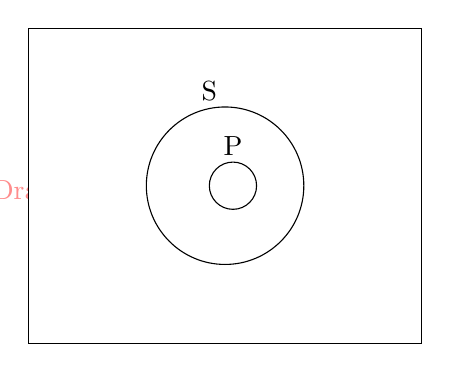
\begin{tikzpicture}
              \filldraw[fill=white] (-2,-2) rectangle (3,2);
              \draw (0.5,0) circle (1)
              (0.6,0) circle (0.3);
              \node at (0.3,1.2) {S};
              \node at (0.6,0.5) {P};
            \end{tikzpicture}
            \label{fig:2.1.2}
          \end{figure}
          令\(S\)为整数,\(P\)为偶数。
        \item
          \begin{figure}[H]
            \centering
            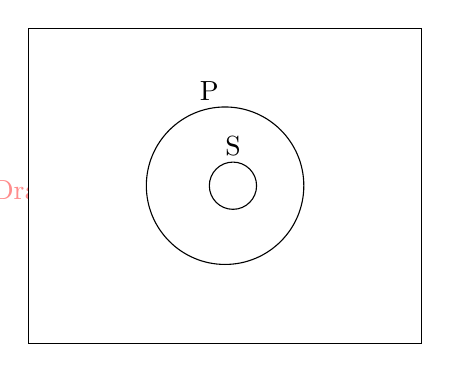
\begin{tikzpicture}
              \filldraw[fill=white] (-2,-2) rectangle (3,2);
              \draw (0.5,0) circle (1)
              (0.6,0) circle (0.3);
              \node at (0.3,1.2) {P};
              \node at (0.6,0.5) {S};
            \end{tikzpicture}
            \label{fig:2.1.3}
          \end{figure}
          令\(S\)为质数,\(P\)为整数。
      \end{itemize}
    \item ``所有\(S\)不是\(P\)''为假,即``有\(S\)为\(P\)''为真。故与上一问相同。
  \end{enumerate}
\end{solution}
\begin{problem}\label{pro:3}
  下列根据对当关系所进行的推理是否有效?为什么?
  \begin{enumerate}
    \item 有些人是画家,所以,有些人不是画家。
    \item 并非所有的办公大楼都是五层的,所以,有些办公大楼不是五层的。
  \end{enumerate}
\end{problem}
\begin{solution}
  \begin{enumerate}
    \item 无效。根据下反对关系,\(I\)假,\(O\)真假不定。
    \item 有效。根据矛盾关系,\(A\)假,\(O\)必真。
  \end{enumerate}
\end{solution}
\begin{problem}\label{pro:4}
  下列直接推理能否成立?如能成立,请用公式写出它的推理过程。
  \begin{enumerate}
    \item 从\(SAP\)真,推出\(\overline{P}O \overline{S}\)真。
    \item 从\(SEP\)真,推出\(\overline{P}I \overline{S}\)真。
  \end{enumerate}
\end{problem}
\begin{solution}
  以下论证均假设主谓项非空。
  \begin{enumerate}
    \item 能成立。由换质法推理可得\(SAP\implies SE \overline{P}\)。
      再由换位法可得\(\overline{P}E S\)。
      再由换质法得\(\overline{P} A \overline{S}\)。
      最后由差等关系推理可得\(\overline{P}I \overline{S}\)。
    \item 不能成立。
  \end{enumerate}
\end{solution}
\begin{problem}\label{pro:5}
  \begin{enumerate}
    \item 请根据换质法和换位法的规则回答,从``一切好的干部都是密切联系群众的''能否推出以下结论:
      \begin{enumerate}
        \item 有些好的干部不是密切联系群众的。
        \item 不密切联系群众的不是好的干部。
        \item 密切联系群众的是好干部。
      \end{enumerate}
      如能,请写出推理形式。如不能,说明理由。
  \end{enumerate}
\end{problem}
\begin{solution}
  \begin{enumerate}
    \item 不能。\(SAP\) 与\(SOP\)是矛盾的。
    \item 能。\(SAP\)由换质法得到\(SE \overline{P}\),再由换位法得到\(\overline{P}ES\),再由换质法得到\(\overline{P}E \overline{S}\).
    \item 不能。\(SAP\)不能得到\(PAS\)。
  \end{enumerate}
\end{solution}
\begin{problem}\label{pro:6}
  下列三段论是否正确?如不正确,违反了哪条规则?
  \begin{enumerate}
    \item 海豚不是鱼,海狮不是海豚,所以,海狮不是鱼。
    \item 甲车间多数工人评上过先进生产者,甲车间有些工人是党员,所以甲车间有
      些党员是先进生产者。
    \item 没有优秀的文艺作品不受群众欢迎的,长篇小说并不都是受群众欢迎的,所
      以,有些长篇小说不是优秀的文艺作品。
  \end{enumerate}
\end{problem}
\begin{solution}
  \begin{enumerate}
    \item 不正确。否定规则。
    \item 不正确。中项不周延。
    \item 正确。
  \end{enumerate}
\end{solution}
\begin{problem}\label{pro:7}
  在括号中填入适当的符号,构成一个正确的三段论,并写出推导过程。
  \begin{enumerate}
    \item \(\begin{matrix}
                   & (\textcolor{white}{M}) & (\textcolor{white}{A}) & (\textcolor{white}{P}) \\
                   & S                      & O                      & M                      \\
        \hline
        \therefore & S                      & (\textcolor{white}{O}) & P                      \\

      \end{matrix}\)
    \item \(\begin{matrix}
                   & (\textcolor{white}{P}) & E                      & (\textcolor{white}{M}) \\
                   & M                      & I                      & S                      \\
        \hline
        \therefore & S                      & (\textcolor{white}{O}) & P                      \\

      \end{matrix}\)
  \end{enumerate}

\end{problem}
\begin{solution}
  \begin{enumerate}
    \item \(\begin{matrix}
                   & ({M}) & ({A}) & ({P}) \\
                   & S     & O     & M     \\
        \hline
        \therefore & S     & ({O}) & P     \\

      \end{matrix}\)

      由于小前提否定知结论一定否定。由\(S\)在小前提中不周延知\(S\)在结论中不周延,故结论为\(SOP\)。
      由中项规则知大前提中中项一定周延。结合否定规则,知大前提必须为\(MAP\)。
    \item \(\begin{matrix}
                   & ({P}) & E     & ({M}) \\
                   & M     & I     & S     \\
        \hline
        \therefore & S     & ({O}) & P     \\

      \end{matrix}\)

      由\(S\)在小前提中不周延,知\(S\)在结论中不周延。结合否定规则,知结论为\(SOP\)。
      显然前提是\(PEM\)。
  \end{enumerate}
\end{solution}
\begin{problem}\label{pro:8}
  请运用三段论有关知识,回答下列问题:
  \begin{enumerate}
    \item 以\(E\)命题为大前提,以\(I\)命题为小前提进行的三段论推理中,结论应该是什么命题?为什么?
    \item 为什么结论是否定命题的三段论式,其大前提不能是\(I\)命题?
  \end{enumerate}
\end{problem}
\begin{solution}
  \begin{enumerate}
    \item 由否定规则知结论为否定命题。由周延规则知结论中小项不周延。故结论应该为\(O\)命题。
    \item 反设大前提可以是\(I\)命题。由否定规则可知小前提为否定命题。由周延规则知大项不周延。
      故结论只可能是\(O\)命题。由中项规则知中项在小前提中周延。故小前提只能是\(SEM\)。
      此时不论大前提是\(PIM\)还是\(MIP\)均不能构成有效三段论。故结论是否定命题的三段论,其大前提不能是\(I\) 命题。
  \end{enumerate}
\end{solution}
\begin{problem}\label{pro:9}
  \begin{enumerate}
    \item 有一个正确的三段论,前提和结论中一共只有三个周延的项,结论中小项
      周延,这是一个怎样的三段论?
    \item 有一个正确的三段论,两个前提中只有大前提中有一个周延的项,这个三
      段论的大前提、小前提和结论各为什么命题?
  \end{enumerate}
\end{problem}
\begin{solution}
  \begin{enumerate}
    \item 中项至少周延一次,结论中小项周延故小前提中小项也周延。故大项均不周延,中项周延恰一次。
      由结论中大项不周延,小项周延,可得结论为\(SAP\)。由结论是肯定的可得大小前提均肯定。
      由小项在小前提周延可得小前提一定为\(SAM\)。故中项在大前提周延,因此大前提一定是\(MAP\)。
    \item 由中项规则知这个项一定是中项。因此大小项在大小前提中都不周延。根据周延规则知大小项在结论中均不周延。
      因此结论只能是\(O\) 命题或者\(I\)命题。
      由中项在大前提周延,大项不周延可知大前提为\(MAP\)。由小前提两项都不周延知小前提只能是\(O\) 命题或者\(I\)命题。
      故所有可能组合为:
      \begin{enumerate}
        \item 结论为\(SOP\),小前提为\(SOM\)。
        \item 结论为\(SIP\),小前提为\(SIM\)。
      \end{enumerate}
      经过验证,这两种可能性都是合法的。
  \end{enumerate}
\end{solution}
\begin{problem}\label{pro:10}
  \begin{enumerate}
    \item 结论是全称命题的正确三段论,其中项不能周延两次。
    \item 已知某有效三段论的大前提为\(O\)命题,证明其小前提必为全称肯定命题,
      并推出这一三段论的格及其形式。
  \end{enumerate}
\end{problem}
\begin{solution}
  \begin{enumerate}
    \item 反设中项周延两次。由结论为全称命题知小项在结论中周延。由周延规则知小项在小前提周延。
      故小前提只能是\(SEM\)。故由否定规则知结论必须否定,因此结论为\(SEP\)。因此\(P\)在结论中周延,
      根据周延规则可知\(P\) 在大前提周延。因此大前提只能为\(PEM\)。这与否定规则是矛盾的。
      因此反设不成立。
    \item 由大前提为\(O\) 命题知中项在大前提不周延。根据中项规则知中项在小前提周延。
      由大前提是否定命题,根据否定规则知小前提是肯定命题,结论是否定命题。
      因此小前提只能是\(MAS\)。由小项在小前提不周延知其在结论不周延。结合结论是否定命题,可得结论一定是\(SOP\)。
      大前提显然是\(POM\)。
  \end{enumerate}
\end{solution}

\end{document}
